\section{Resultados del Laboratorio}

El trabajo experimental realizado en el laboratorio consiste en comprobar cada uno de los requisitos de prueba propuestos en el preinforme, los cuales suelen ser actualizados durante el desarrollo de la experiencia. Por lo anterior, en este informe se han actualizado los valores de ciertos componentes, basados en el correcto funcionamiento de los requisitos de prueba.

\vspace{0.4cm}

\begin{figure}[h]
    \Centering
    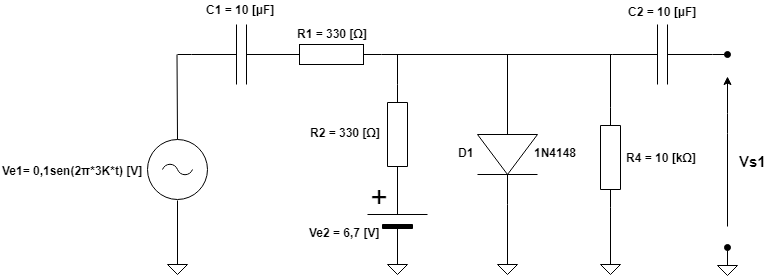
\includegraphics[scale=0.57]{Imagenes/7Resultados/circuites-inf3.png}
    \caption{Circuito implementado para análisis}
	\label{fig:figure9}
\end{figure}

\vspace{.4 cm}
En la Figura \ref{fig:figure9} podemos ver el circuito implementado para el desarrollo de esta experiencia, incluyendo los valores de cada componente.\\
Entendiendo que el circuito presentado corresponde a la unión del Módulo 1 (Figura \ref{fig:figure3}) y Módulo 2 (Figura \ref{fig:figure4}), se describirán las estrategias de resolución de los Requisitos de Prueba según el módulo que sea requerido.
\vspace{.2 cm}

\centering
\extrarowheight = -0.5ex
\renewcommand{\arraystretch}{2.25}
\begin{tabular}{p{0.1\textwidth} p{0.9\textwidth}}

\textbf{RP1} & Para este requisito se ha trabajado con dos diodos, 1n4148 y 1n4070, los cuales se examinaron por separado con la ayuda de una resistencia variable. Con el tester digital se midió el voltaje (V$_{D1}$) y la corriente (I$_{D1}$) que pasan por el diodo D1 mientras se variaba el voltaje continuo. En función de hacer una curva más detallada, en la cual sea evidente el comportamiento característico de los diodos, se realizó una gran cantidad de mediciones continuas de V$_{D1}$ e I$_{D1}$.  %(INSERTAR GRÁFICO Y TABLA DE MEDICIONES DE NICO)
\\ 

\end{tabular}


\begin{table}[h]
\resizebox{\textwidth}{!}{%
\begin{tabular}{|c|c|c|c|c|c|c|c|c|c|c|c|c|c|c|c|c|c|c|}
\hline
\textbf{VD {[}mV{]}} & 555 & 589 & 623 & 654 & 668 & 695 & 715 & 731 & 759 & 773 & 791 & 815 & 832 & 842 & 848 & 854 & 857 & 857 \\ \hline
\textbf{ID {[}mA{]}} & 0.5 & 1   & 2   & 3.8 & 5.1 & 9.1 & 14  & 20  & 40  & 56  & 99  & 175 & 260 & 378 & 500 & 769 & 840 & 895 \\ \hline
\end{tabular}%
}
\caption{Datos de Corriente y Voltaje por diodo 1N4007}
\label{my-label}
\end{table}

\newpage
\begin{figure}[h]
    \Centering
    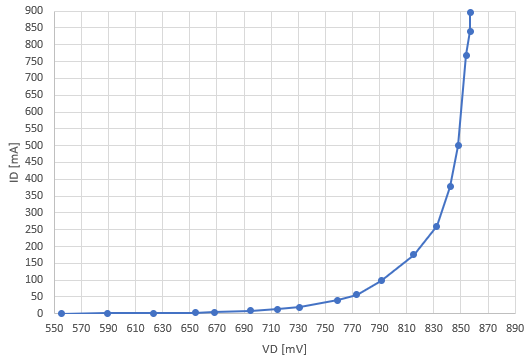
\includegraphics[scale=0.55]{Imagenes/7Resultados/diodo1n4007.png}
    \caption{Gráfico ID v/s VD Diodo 1N4007}
	\label{fig:figure10}
\end{figure}

\begin{table}[h]
\resizebox{\textwidth}{!}{%
\begin{tabular}{|c|c|c|c|c|c|c|c|c|c|c|c|c|c|c|c|c|c|}
\hline
\textbf{VD {[}mV{]}} & 585 & 618 & 649 & 680 & 720 & 730 & 735 & 786 & 797 & 807 & 826 & 844 & 892 & 937 & 943 & 961 & 997 \\ \hline
\textbf{ID {[}mA{]}} & 0.5 & 1   & 2   & 3.8 & 6   & 7   & 8   & 21  & 24  & 28  & 36  & 47  & 78  & 117 & 126 & 150 & 176 \\ \hline
\end{tabular}%
}
\caption{Datos de Corriente y Voltaje por diodo 1N4148}
\label{my-label}
\end{table}

\begin{figure}[h]
    \Centering
    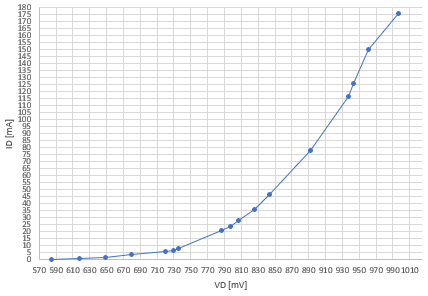
\includegraphics[scale=0.55]{Imagenes/7Resultados/diodo1n4148.png}
    \caption{Gráfico ID v/s VD Diodo 1N4148}
	\label{fig:figure10}
\end{figure}

\centering
\extrarowheight = -0.5ex
\renewcommand{\arraystretch}{2.25}
\begin{tabular}{p{0.1\textwidth} p{0.9\textwidth}}
\textbf{RP2} & Considerando el circuito completo, para poder demostrar que los valores de las capacitancias escogidas tienen carácter despreciable en el análisis de nuestra experiencia, debemos ver el desfase que pueden provocar los condensadores entre la señal alterna de entrada y la de salida. Por ello, se han medido las señales mencionadas, y podemos ver en la Figura \ref{fig:figure11} que no hay desfase entre ellas, por lo que el requisito queda demostrado. \\ 

\end{tabular}

\begin{figure}[h]
    \Centering
    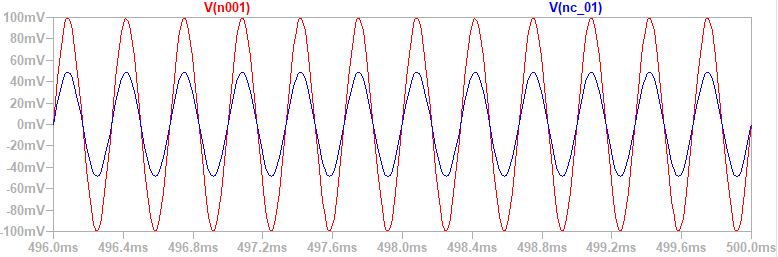
\includegraphics[scale=0.6]{Imagenes/7Resultados/ve1vs1.PNG}
    \caption{Señal alterna Ve1 y Ve2}
	\label{fig:figure11}
\end{figure}

\centering
\extrarowheight = -0.5ex
\renewcommand{\arraystretch}{2.25}
\begin{tabular}{p{0.1\textwidth} p{0.9\textwidth}}

\textbf{RP3} & Para este requisito se trabaja únicamente con el MOD 1, estableciendo un Voltaje Va, que se encuentra paralelo a la resistencia R2 y la fuente continua Ve2.\\
& Con la configuración propuesta en la descripción del requisito, medimos el voltaje alterno de salida en circuito abierto (Voltaje Thévenin VTca), como muestra la Figura \ref{fig:figure13}. El valor obtenido fue de \textbf{VTca = 46 [mV].} \\ 
\end{tabular}

\begin{figure}[h]
    \Centering
    \includegraphics[scale = 0.35]{Imagenes/7Resultados/vtca.png}
    \caption{Voltaje Thévenin alterno entre terminal a y tierra}
	\label{fig:figure13}
\end{figure}

\centering
\extrarowheight = -0.5ex
\renewcommand{\arraystretch}{2.25}
\begin{tabular}{p{0.1\textwidth} p{0.9\textwidth}}

& Para obtener la impedancia del equivalente Thévenin del MOD 1 sin apagar la fuente, utilizamos el modelo planteando en la Figura \ref{fig:figure14}.\\
\end{tabular}

\begin{figure}[h!]
    \Centering
    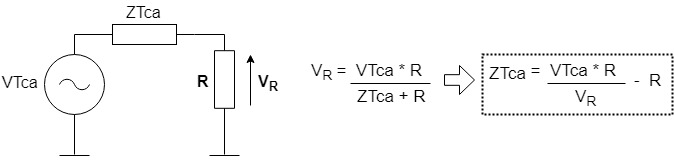
\includegraphics[scale=0.6]{Imagenes/6Analisis/divT.jpg}
    \caption{Divisor de Tensiones para $ZTH_{ca}$}
	\label{fig:figure14}
\end{figure}
\newpage
\centering
\extrarowheight = -0.5ex
\renewcommand{\arraystretch}{2.25}
\begin{tabular}{p{0.1\textwidth} p{0.9\textwidth}}

& Entonces, configurando el circuito con el modelo planteado, conectamos una resistencia R = 330 [$\Omega$], con voltaje V$_{R}$ = 30,4 [mV]. Por lo anterior, el resultado de ZTca para esta experiencia es: 
\[ ZTca = \frac{0,46 * 330}{0,304} - 330 = \mathbf{169,34 [\Omega]} \hspace{0.2cm} (\geq 85[\Omega] )
\]
\\ 

\textbf{RP4} & Para este requisitos hemos de trabajar con el circuito completo, es decir, ambos módulos conectados. \\
& Una vez configurado el circuito según la descripción de RP3, y obtenida la curva característica en la Figura \ref{fig:figure10}, con la fuente de poder variamos la corriente de entrada del tal forma que a través del diodo atraviesen los siguientes valores: \\
\end{tabular}

\begin{figure}[H]
\centering
\begin{minipage}[c]{0.4\linewidth}
\centering
    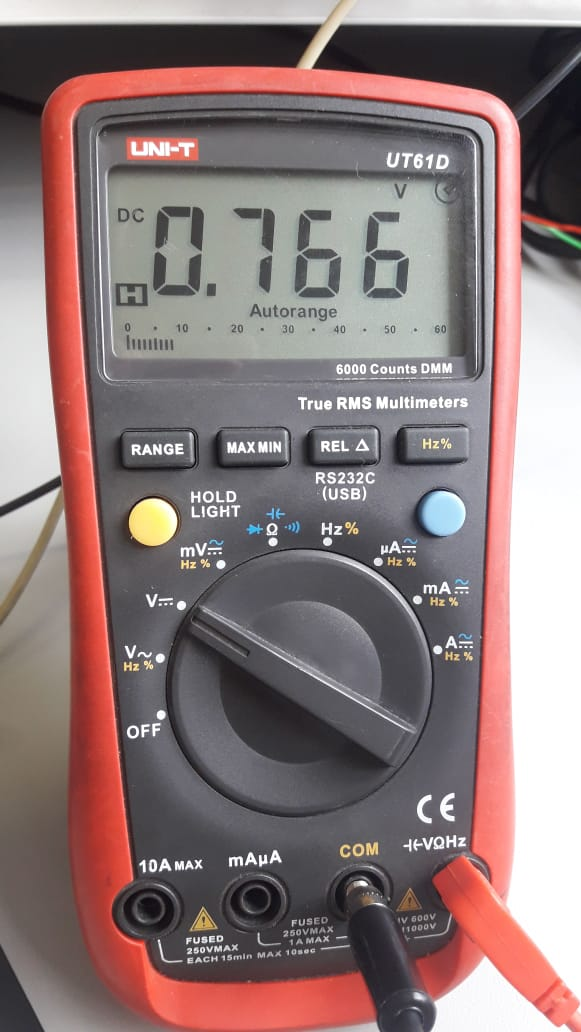
\includegraphics[scale=0.22]{Imagenes/7Resultados/Vdiodo.jpeg}
    \caption{Voltaje a través del diodo}
    \label{fig:figura1}
\end{minipage}
\hspace{0.25cm}
\begin{minipage}[c]{0.4\linewidth}
\centering
    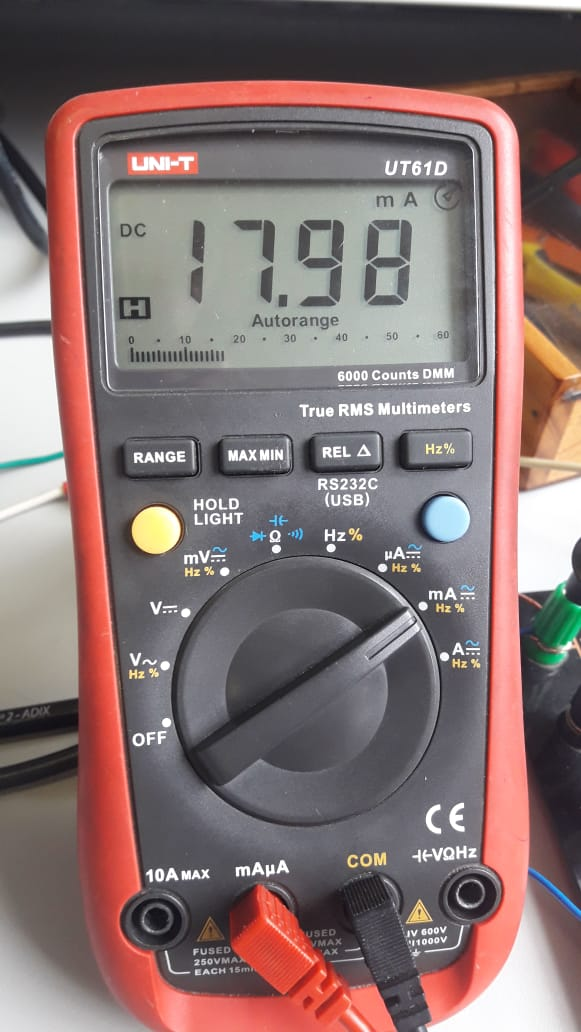
\includegraphics[scale=0.22]{Imagenes/7Resultados/Idiodo.jpeg}
    \caption{Corriente a través del diodo}
    \label{fig:figura2}
\end{minipage}
\end{figure}

\centering
\extrarowheight = -0.5ex
\renewcommand{\arraystretch}{2.25}
\begin{tabular}{p{0.1\textwidth} p{0.9\textwidth}}
& De esta forma queda definido el punto de operación Q con los valores presentados en las Figuras 11 y 12. 
\\ 

\textbf{RP5} & La resistencia dinámica del diodo en el punto Q se define de la siguiente manera:
\[ R_{D} = \frac{V_{DQ}}{I_{DQ}} = \frac{0.766}{0.01798} \approx 42,6 [\Omega]
\]
EL valor de R4 escogido es de 10[k$\Omega$], que cumple con $R4 >> 10 * R_{D}$.
\\

\textbf{RP6} & Para este requisito, se debe trabajar directamente con los requisitos funcionales, por lo tanto, para encontrar las constantes k y n nos dedicaremos a comprobar RF1 y RF2.
\end{tabular}

\newpage
\RaggedRight
\textbf{Prueba de Requisitos Funcionales} 
\\
\vspace{0.7cm}

\centering
\extrarowheight = -0.5ex
\renewcommand{\arraystretch}{2.25}
\begin{tabular}{p{0.1\textwidth} p{0.9\textwidth}}

\textbf{RF1} & En este requisito se trabaja sólo con el MOD1. Para observar la comparación de ambas señales, se realizó la simulación por LTSpice del MOD1, y de él se midió la señal entre los terminales de salida (ante la ausencia de dicha imagen, que se realizó en el laboratorio), del cual se obtuvo la señal que observamos en la Figura 15. Dicha señal corresponde al voltaje alterno de la señal Va, y esta oscila entre 125 [mV] y 223[mV]. 
\\
\end{tabular}

\begin{figure}[H]
\centering
\begin{minipage}[c]{0.4\linewidth}
\centering
    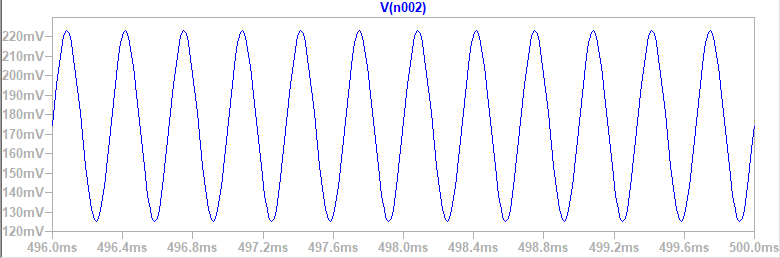
\includegraphics[scale=0.25]{Imagenes/7Resultados/Va.PNG}
    \caption{Señal de salida alterna de Va, MOD1}
    \label{fig:figura14}
\end{minipage}
\hspace{1.7cm}
\begin{minipage}[c]{0.4\linewidth}
\centering
    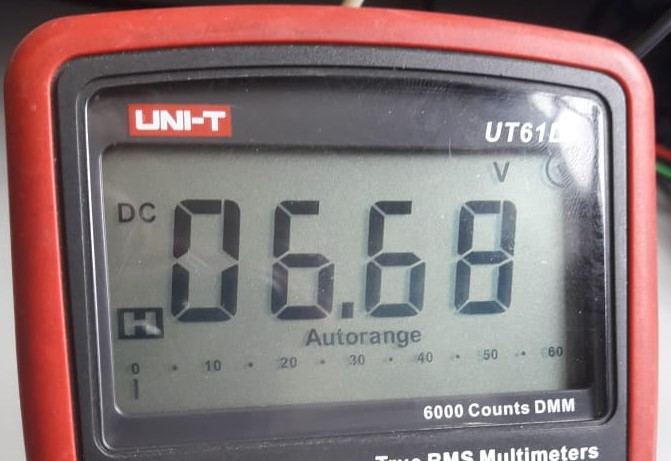
\includegraphics[scale=0.15]{Imagenes/7Resultados/Vcc.jpeg}
    \caption{Señal de salida continua de Va, MOD1}
    \label{fig:figura15}
\end{minipage}
\end{figure}

\centering
\extrarowheight = -0.5ex
\renewcommand{\arraystretch}{2.25}
\begin{tabular}{p{0.1\textwidth} p{0.9\textwidth}}
& La Figura 16 muestra el voltaje continuo medido con el tester digital para este módulo. \\
& De lo anterior, se concluye que $Va = 6,68 + 0,174sen(wt)[V]$, y podemos observar que el voltaje alterno de salida difiere en pequeñas magnitudes al voltaje alterno de entrada, por lo tanto, tomando en cuenta el detalle de los datos, el valor obtenido de la constante \textbf{k = 1,74}. 
\\
\end{tabular}
\vspace{0.6cm}

\centering
\extrarowheight = -0.5ex
\renewcommand{\arraystretch}{2.25}
\begin{tabular}{p{0.1\textwidth} p{0.9\textwidth}}
\textbf{RF2} & Este requisito define Vs1 = n*Ve1, para todo el circuito. Este requisito nos plantea un n variable, que dependerá de los valores que vayamos ingresando a la fuente continua Ve2.\\

& En la tabla \ref{Table2} se adjunta la "Tabla de Valores", obtenida luego de realizar varias mediciones al circuito, de la cual obtenemos distintos valores para n según vamos variando Ve2.
\end{tabular}

\begin{table}[h]
\centering
\caption{Tabla de Valores para n}
\label{Table2}
\begin{tabular}{@{}|c|c|c|c|c|@{}}
\toprule
Ve2 {[}V{]} & Idq {[}mA{]} & Vdq {[}V{]} & Vs1 pp {[}mV{]} & n \\ \midrule
6 & 0,756 & 5,34 & 2 & 0,01 \\
5 & 0,744 & 4,3 & 2,5 & 0,0125 \\
4 & 0,729 & 3,3 & 3 & 0,015 \\
3 & 0,710 & 2,36 & 4 & 0,02 \\
2 & 0,684 & 1,4 & 6 & 0,03 \\
1 & 0,624 & 0,499 & 16 & 0,08 \\
0,5 & 0,538 & 0,089 & 52 & 0,26 \\ \midrule
\textbf{0,18} & 0,157 & 0,021 & 97,8 & \textbf{0,489} \\ \bottomrule
\end{tabular}
\end{table}
\\ 

\centering
\extrarowheight = -0.5ex
\renewcommand{\arraystretch}{2.25}
\begin{tabular}{p{0.1\textwidth} p{0.9\textwidth}}
& De la tabla, destacamos el último valor de Ve2, que corresponde al ajuste del circuito que nos pide RP6, de modo que \textbf{ n = 0,489 $\approx$ 0,5}. Y con esta última prueba, quedan todos los Requisitos planteados durante el desarrollo de la experiencia y el informe verificados. \\
\end{tabular}
\\
\\
\\
\newpage

 